\documentclass{article}

\usepackage{graphicx}
\usepackage{tikz}
\usepackage{tikzsymbols}
\usetikzlibrary{calc,patterns,shapes.geometric}
\pagestyle{empty}
\usepackage[margin=0pt]{geometry}
\geometry{papersize={14in,12in}}

\def\centerarc[#1](#2)(#3:#4:#5){\draw[#1] ($(#2)+({#5*cos(#3)},{#5*sin(#3)})$) arc (#3:#4:#5);}

\begin{document}
	\begin{figure}
		\centering
		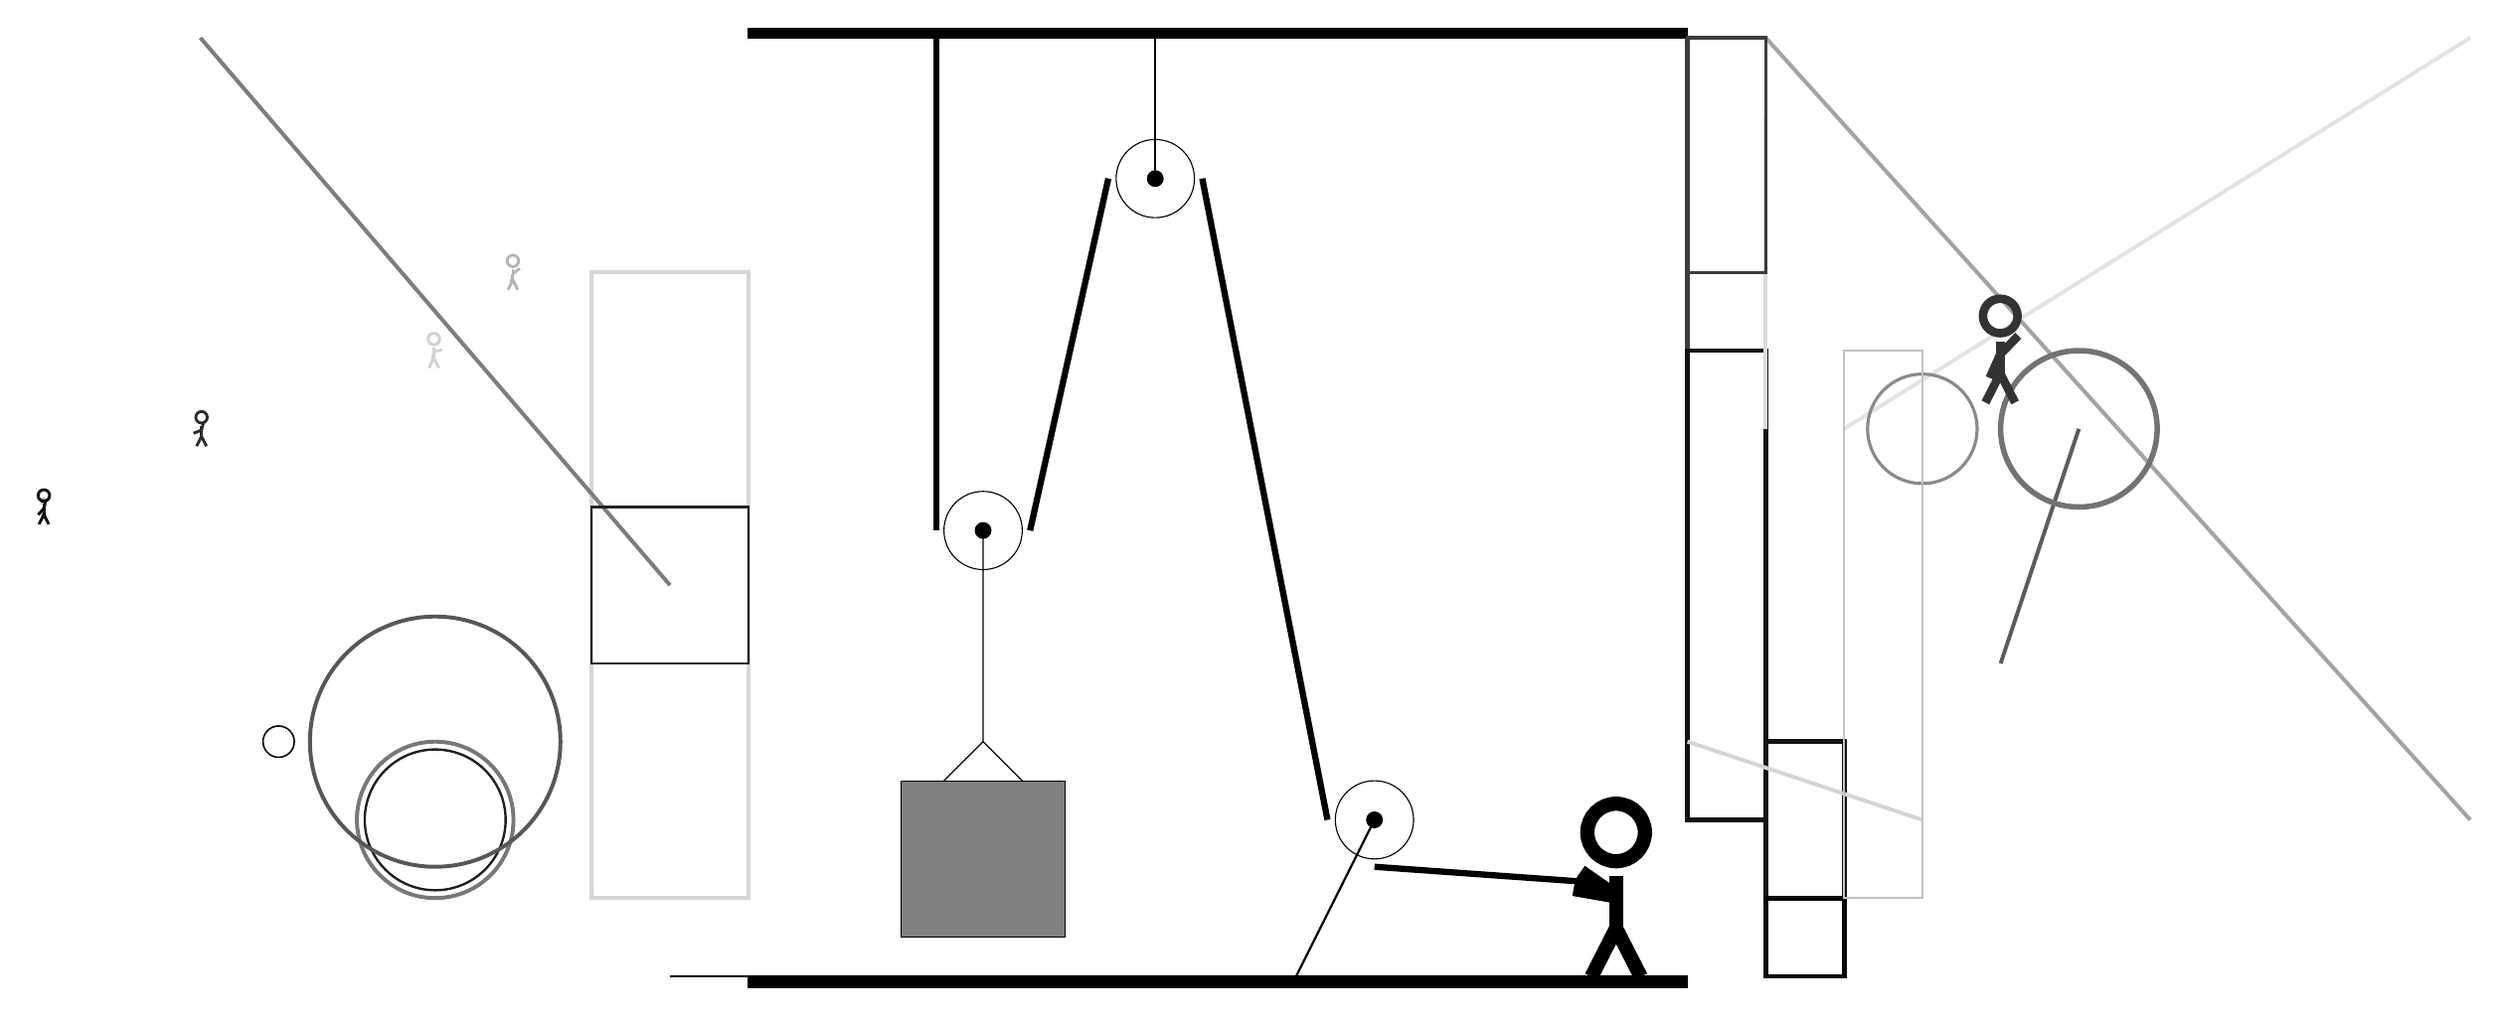
\begin{tikzpicture}
			%%%%% START %%%%%
			
			\draw[fill=black] (-2, 9) rectangle (10, 9.125);
			
			\draw (3.2, 7.2) circle (0.5);
			\draw[fill=black] (3.2, 7.2) circle (0.1);
			\draw[thick] (3.2, 7.2) -- (3.2, 9);
			
			\draw (6, -1) circle (0.5);
			\draw[fill=black] (6, -1) circle (0.1);
			\draw[thick] (6, -1) -- (5, -3);
			
			\draw (1, 2.7) circle (0.5);
			\draw[fill=black] (1, 2.7) circle (0.1);
			
			\draw[line width=0.5mm, color=black!64](15, 4) -- (14, 1);
			
			\draw[line width=0.5mm, color=black!16] (-4, 6) rectangle (-2, -2);
			\draw [line width=0.3mm, color=black!88](-6, -1) circle (0.9);
			\draw[line width=0.5mm, color=black!36](11, 9) -- (20, -1);
			
			\draw[line width=0.6mm, color=black!76] (10, 1) rectangle (10, 9);
			
			\draw[line width=0.6mm, color=black!93] (10, -1) rectangle (11, 5);
			
			\draw[line width=0.5mm, color=black!14](11, 8) -- (11, 4);
			\node[line width=0.3mm, color=black!35] at (-11, 3) {\Strichmaxerl[1][62][45]};
			\draw[line width=0.6mm, color=black!92] (12, -3) rectangle (11, 0);
			
			\draw [line width=0.5mm, color=black!53](-6, -1) circle (1.0);
			\draw[line width=0.4mm, color=black!76] (10, 9) rectangle (11, 6);
			\node[line width=0.4mm, color=black!94] at (-11, 3) {\Strichmaxerl[2][49][78]};
			\draw[line width=0.6mm, color=black!97] (11, -3) rectangle (12, -2);
			
			\node[line width=0.7mm, color=black!18] at (-6, 5) {\Strichmaxerl[2][79][15]};
			\draw[line width=0.5mm, color=black!11](12, 4) -- (20, 9);
			\draw[line width=0.5mm, color=black!17](13, -1) -- (10, 0);
			
			\draw [line width=0.5mm, color=black!66](-6, 0) circle (1.6);
			\draw [line width=0.4mm, color=black!46](13, 4) circle (0.7);
			\draw[line width=0.5mm, color=black!51](-3, 2) -- (-9, 9);
			\draw[line width=0.3mm, color=black!86] (-4, 3) rectangle (-2, 1);
			\draw[line width=0.3mm, color=black!99] (-3, -3) rectangle (-2, -3);
			
			\draw[line width=0.2mm, color=black!24] (12, -2) rectangle (13, 5);
			\draw [line width=0.7mm, color=black!55](15, 4) circle (1.0);
			\draw [line width=0.2mm, color=black!98](-8, 0) circle (0.2);
			\node[line width=0.7mm, color=black!29] at (-5, 6) {\Strichmaxerl[2][79][37]};
			
			\node[line width=0.6mm, color=black!80] at (14, 5) {\Strichmaxerl[6][66][46]};
			\node[line width=0.6mm, color=black!83] at (-9, 4) {\Strichmaxerl[2][22][75]};
			
			\draw (1, 2.7) -- (1, 0) -- (0.5, -0.5);
			\draw (1, 0) -- (1.5, -0.5);
			\draw[fill=black!50] (-0.05, -0.5) rectangle (2.05, -2.5);
			
			\draw[line width=0.8mm] (0.4, 9) -- (0.4, 2.7);
			\centerarc[line width=0.8mm](1, 2.7)(180:360:0.6);
			\draw[line width=0.8mm](1.6, 2.7) -- (2.6, 7.2);
			\centerarc[line width=0.8mm](3.2, 7.2)(0:180:0.6);
			\draw[line width=0.8mm](3.8, 7.2) -- (5.4, -1);
			\centerarc[line width=0.8mm](6, -1)(180:270:0.6);
			\draw[line width=0.8mm](6, -1.6) -- (8.8, -1.8);
			
			\node at (9, -1.9) {\Strichmaxerl[10][-35][170]};
			
			\draw[fill=black] (-2, -3) rectangle (10, -3.15);
			
			%%%%% END %%%%%
		\end{tikzpicture}
	\end{figure}	
\end{document}